\documentclass
[12pt,a4paper]
{article}

% Packages
\usepackage{amsmath}
\usepackage{graphicx}
\usepackage{hyperref}
\usepackage{booktabs}
\usepackage{verbatim}
\usepackage{geometry}
\geometry{left=2cm}
\geometry{right=1.5cm}
\geometry{top=1cm}
\geometry{bottom=2cm}


% Document information
\title{Protocol of RF Detector Calibration}
\author{IAP RAS}
\date{\today}

\begin{document}

\maketitle

\section{Measurement equipment}


\begin{enumerate}
    \item Microwave generator: \texttt{Rigol DSG830}
    \item Spectrum analyzer: \texttt{Rigol RSA5065N}
    \item Oscilloscope: \texttt{Tektronix MDO34}
\end{enumerate}

\section{Parameters}
Parameters from DetCal settings file shown below.

\begin{table}[htbp]
\centering
\begin{tabular}{|c|c|}
\hline
RF frequencies & [2450000000.0, 0.0, 1] \\
\hline
RF levels & [-5.0, 15.0, 51] \\
\hline
SPAN wide & 2000000.0 \\
\hline
SPAN narrow & 100000.0 \\
\hline
RBW wide & 10000.0 \\
\hline
RBW narrow & 1000.0 \\
\hline
VBW wide & 10000.0 \\
\hline
VBW narrow & 1000.0 \\
\hline
REF level & 15.0 \\
\hline
SWEEP points & 1001.0 \\
\hline
SWEEP time & AUTO ON \\
\hline
Precise & True \\
\hline
HOR scale & 0.01 \\
\hline
High res & True \\
\hline
Impedance 50Ohm & True \\
\hline
Coupling DC & True \\
\hline
Channel & 4 \\
\hline
\end{tabular}
\caption{Measurement parameters}
\label{params}
\end{table}

\newpage
\section{Results}


\begin{figure}[htbp]
\centering
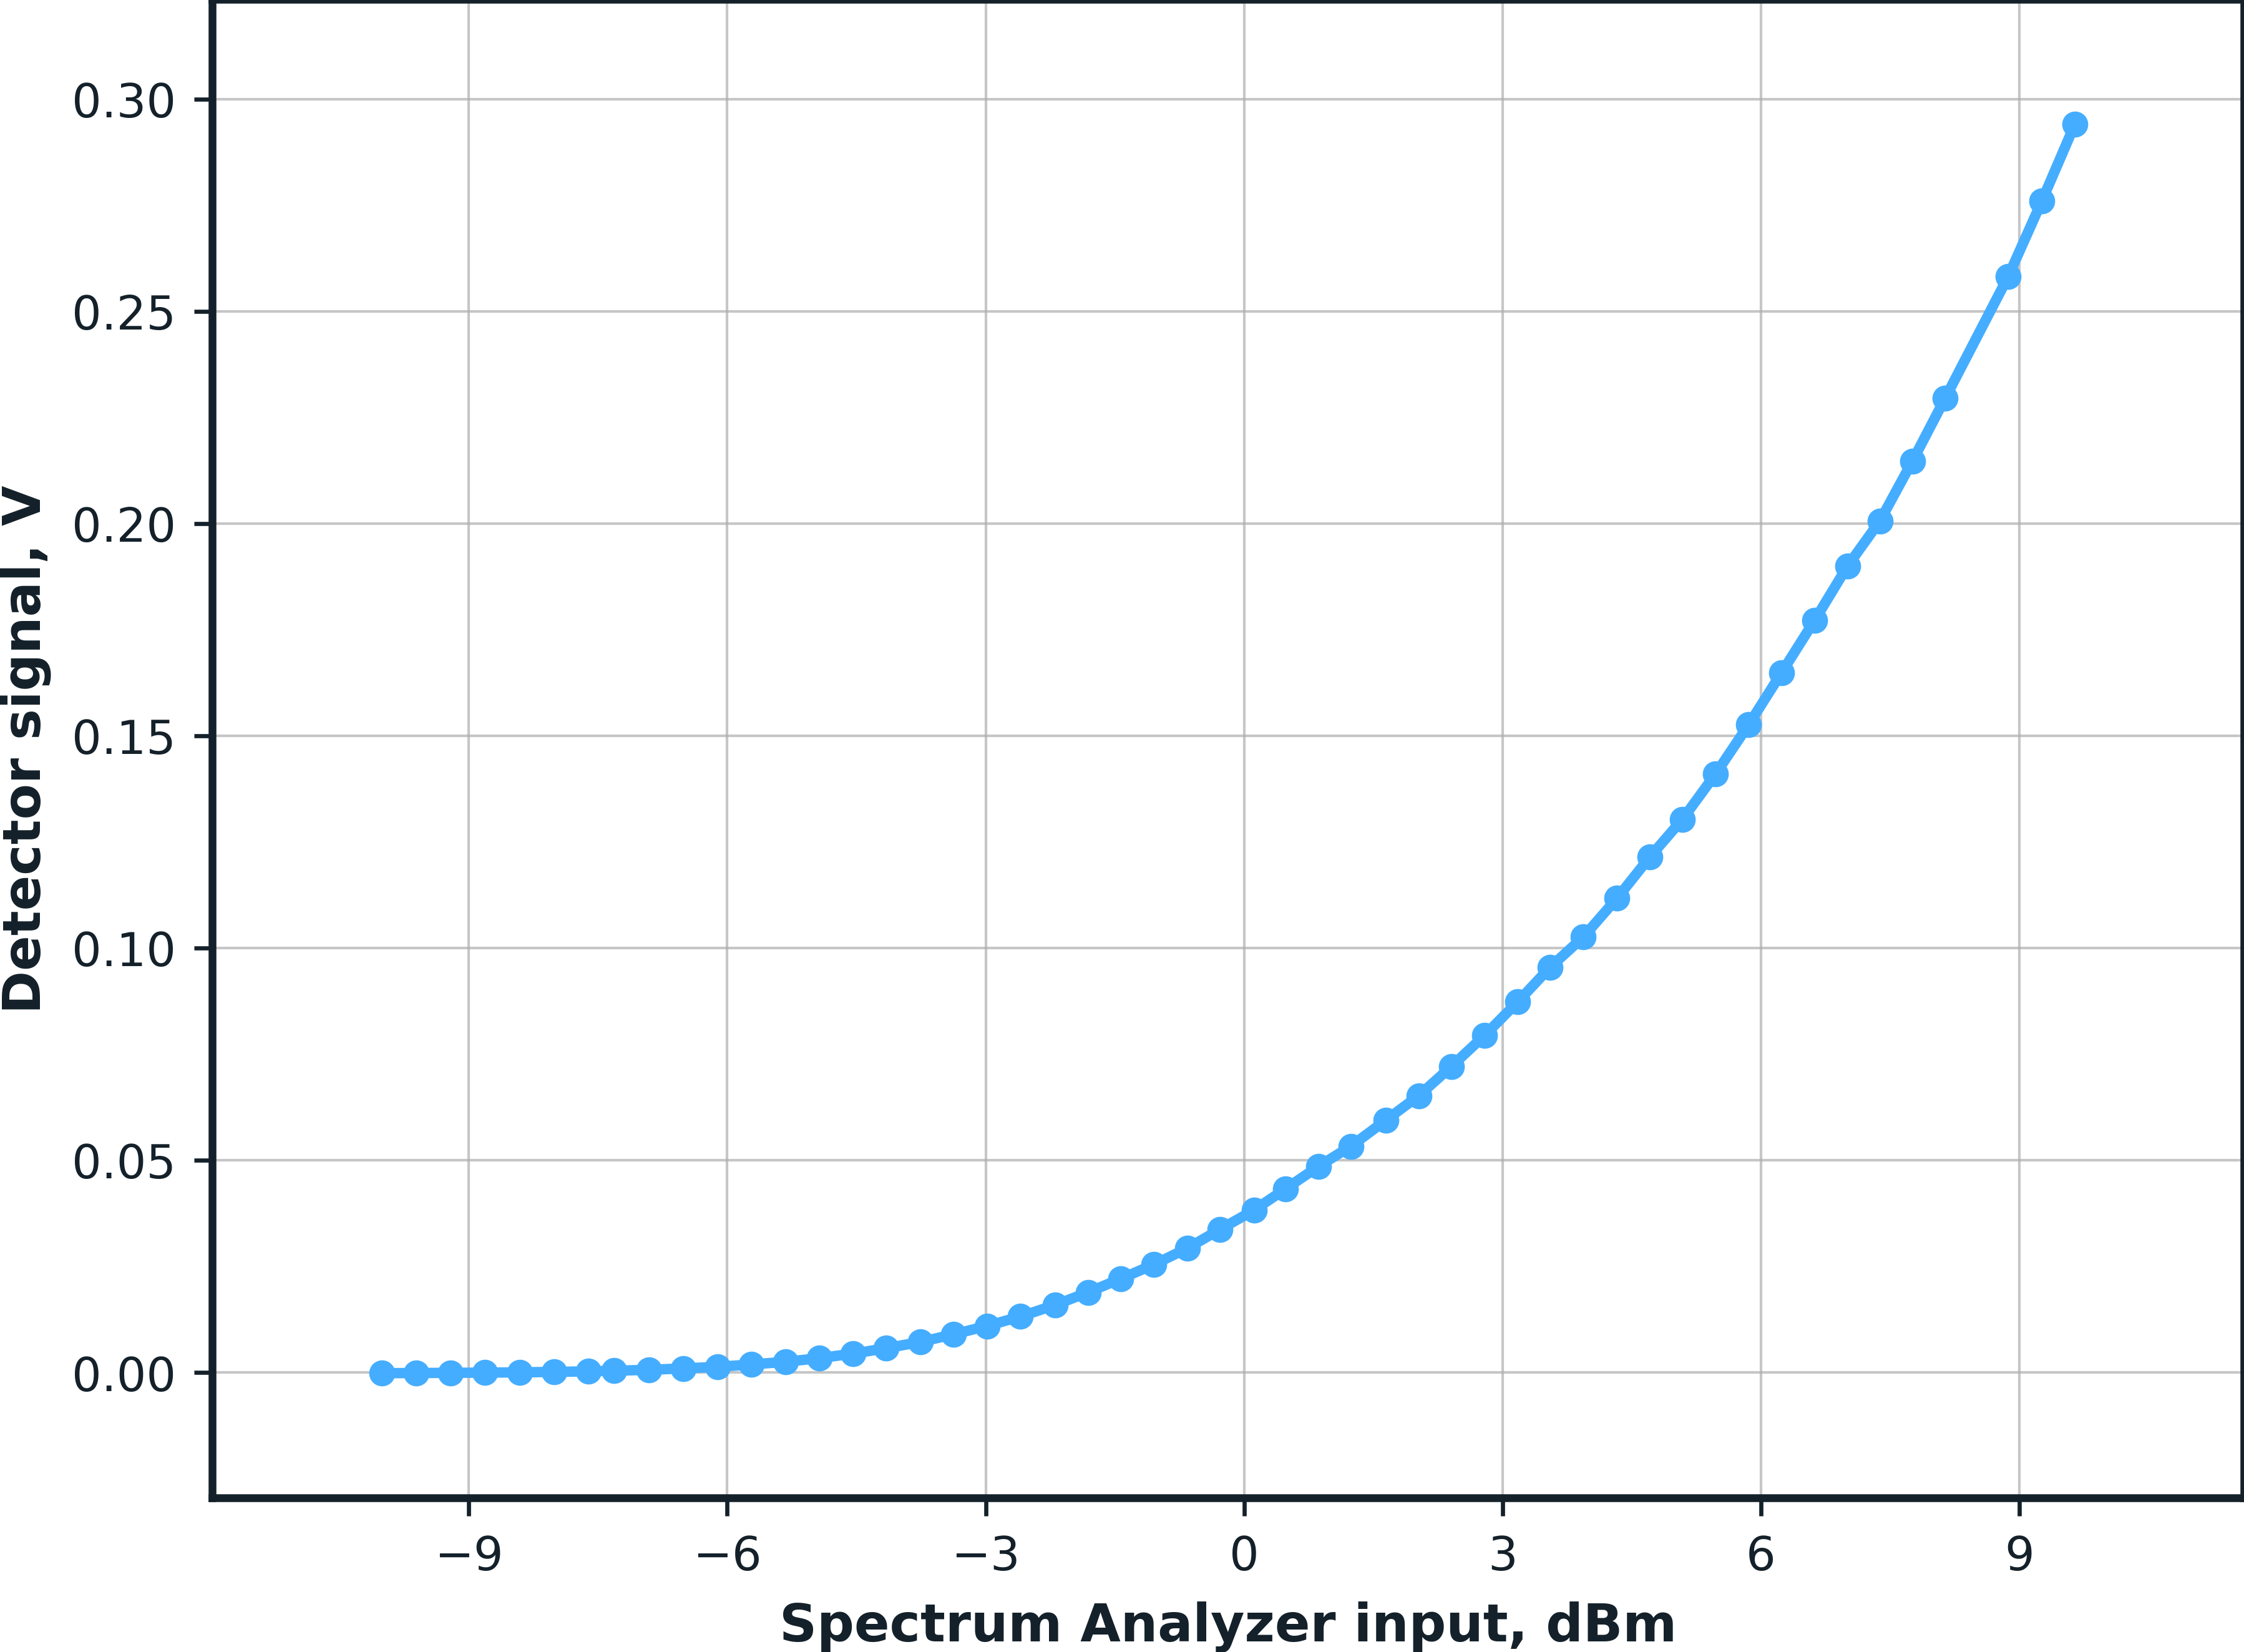
\includegraphics[width=1.0\textwidth]{measurement_data.png}
\caption{Detector response at 2450.00 MHz}
\label{Figure}
\end{figure}

\end{document}